\documentclass{beamer}

\usepackage{pgfplots}
\usepackage{appendixnumberbeamer}
\usepackage{multirow}

\usetheme{metropolis}

%Catalogue
%Viridis
\definecolor{viridis0}{rgb}{0.28, 0.13, 0.45}
\definecolor{viridis1}{rgb}{0.26, 0.24, 0.52}
\definecolor{viridis2}{rgb}{0.22, 0.34, 0.55}
\definecolor{viridis3}{rgb}{0.18, 0.44, 0.56}
\definecolor{viridis4}{rgb}{0.14, 0.52, 0.56}
\definecolor{viridis5}{rgb}{0.12, 0.61, 0.54}
\definecolor{viridis6}{rgb}{0.17, 0.69, 0.5}
\definecolor{viridis7}{rgb}{0.32, 0.77, 0.41}
\definecolor{viridis8}{rgb}{0.53, 0.83, 0.29}
\definecolor{viridis9}{rgb}{0.76, 0.88, 0.14}

%Catalogue
\definecolor{custom_one}{HTML}{00a0b0}
\definecolor{custom_two}{HTML}{eb6841}
\definecolor{custom_three}{HTML}{cc2a36}
\definecolor{custom_four}{HTML}{4f372d}
\definecolor{custom_five}{HTML}{183059}
\definecolor{custom_six}{HTML}{edc951}

\definecolor{custom_one}{HTML}{edc951}
\definecolor{custom_two}{HTML}{eb6841}
\definecolor{custom_three}{HTML}{cc2a36}
\definecolor{custom_four}{HTML}{4f372d}
\definecolor{custom_five}{HTML}{00a0b0}

\title{Human Age Prediction Based on Real and Simulated RR Intervals using Temporal Convolutional Neural Networks and Gaussian Processes}
\date{\today}
\author{Maximilian Pfundstein (maxpf364)}
\institute{Linköpings University}

\setbeamertemplate{frame footer}{Master Thesis (732A64)}

\begin{document}
    \maketitle
    
    \begin{frame}{Table of contents}
      \setbeamertemplate{section in toc}[sections numbered]
      \tableofcontents%[hideallsubsections]
    \end{frame}
    
    \section{Recap}
    \begin{frame}{Recap | Age Prediction}
        \begin{figure}[hbt]
        	\center
        	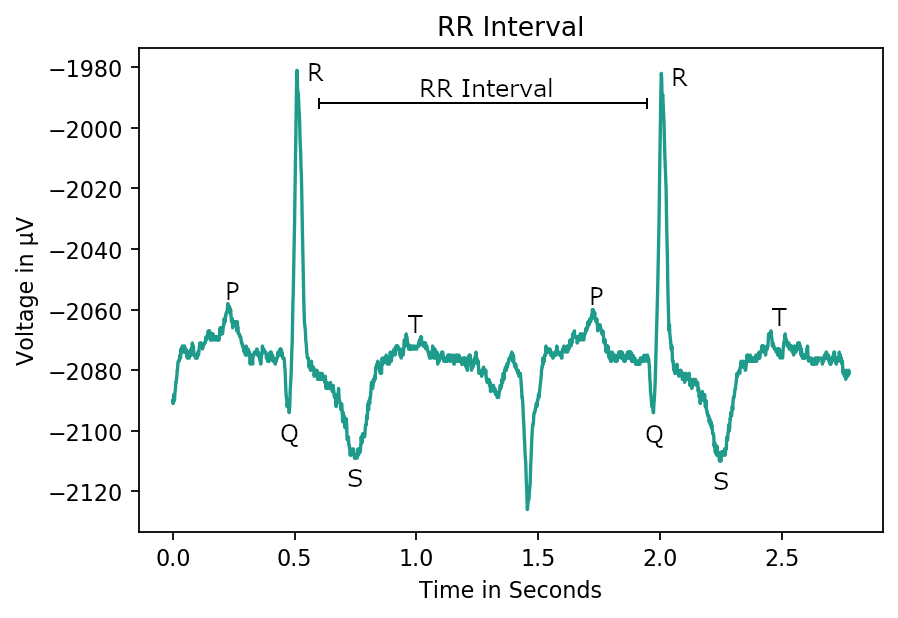
\includegraphics[width=1.0\textwidth]{img/rr-interval.png}
        	%\caption{}
        	\label{fig:rr}
        \end{figure}
    \end{frame}
    
    \begin{frame}{Recap | Data Sets | Gdańsk}
        \begin{figure}[hbt]
        	\center
        	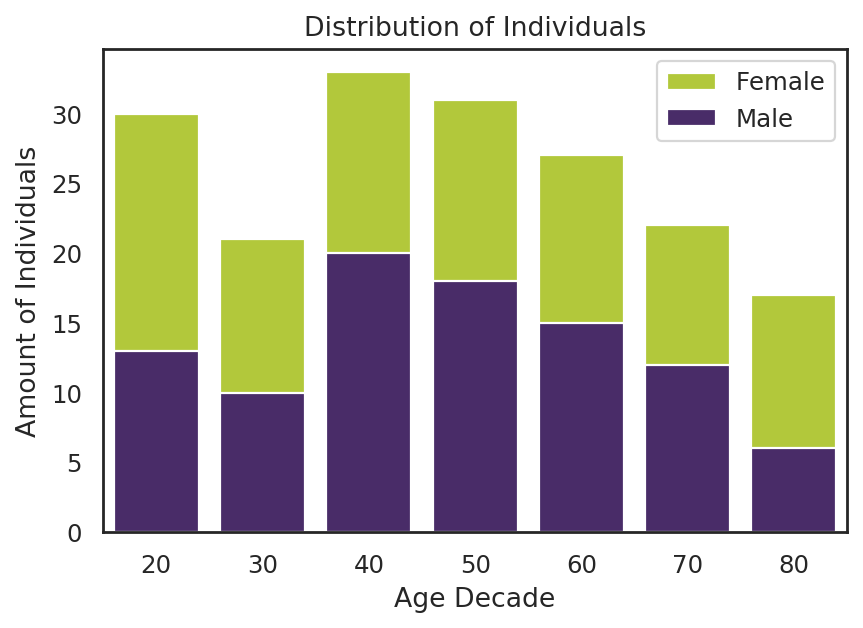
\includegraphics[width=1.0\textwidth]{img/gdansk-distribution-subjects.png}
        	%\caption{}
        	\label{fig:dist_gdansk}
        \end{figure}
    \end{frame}
    
    \begin{frame}{Recap | Data Sets | PhysioNet}
        \begin{figure}[hbt]
        	\center
        	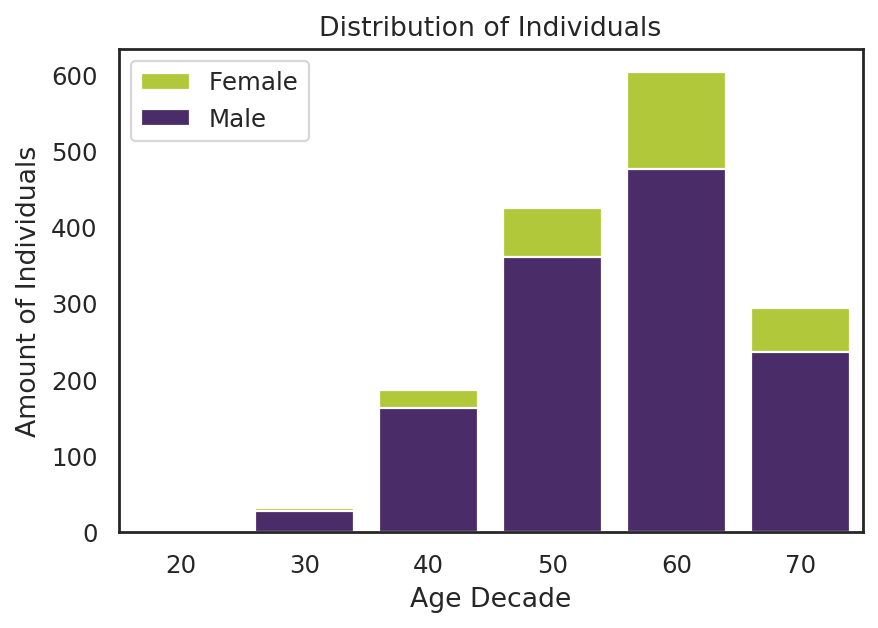
\includegraphics[width=1.0\textwidth]{img/physionet-distribution-subjects.png}
        	%\caption{}
        	\label{fig:dist_physionet}
        \end{figure}
    \end{frame}
    
    \begin{frame}{Recap | Impurity and Padding}
        \begin{figure}[hbt]
        	\center
        	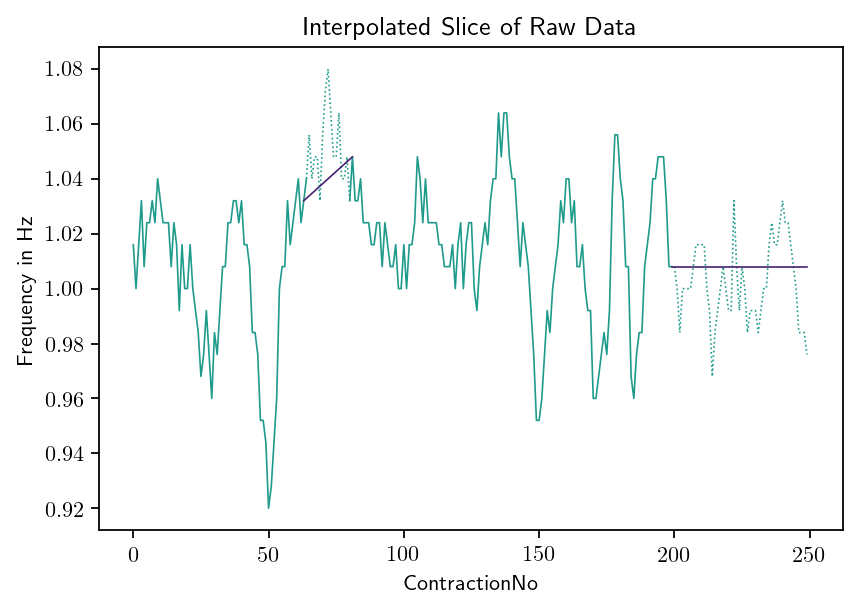
\includegraphics[width=1.0\textwidth]{img/slice_raw_data_linear_spline_interpolation.png}
        	%\caption{}
        	\label{fig:interpolation_and_padding}
        \end{figure}
    \end{frame}
    
    \section{Methods and Models}
    \begin{frame}{Methods and Models | Methods}
        \begin{itemize}
            \item \textit{complete} and \textit{constant}
            \begin{itemize}
                \item 48 slices of around 5 minutes
            \end{itemize}
            \item \textit{classification} and \textit{regression}
            \begin{itemize}
                \item classes have no order
            \end{itemize}
            \item 33 features as used in a previous paper (\texttt{hrvanalysis})
        \end{itemize}
    \end{frame}
    
    \begin{frame}{Methods and Models | Feature Based Models}
        \begin{itemize}
            \item Naive Bayes
            \item Support Vector Machines
            \begin{itemize}
                \item Hyperparameters
                \begin{itemize}
                    \item Classification: $\gamma_C$ (kernel length scale), $C_C$ (regularisation)
                    \item Regression: $\gamma_R$ (kernel length scale), $C_R$ (regularisation), $\epsilon_R$ (slack)
                \end{itemize}
                \item 5 fold cross-validation
            \end{itemize}
            \item Random Forest
            \item XGBoost
        \end{itemize}
    \end{frame}
    
    \begin{frame}{Methods and Models | Convolution}
        \begin{figure}[hbt]
        	\center
        	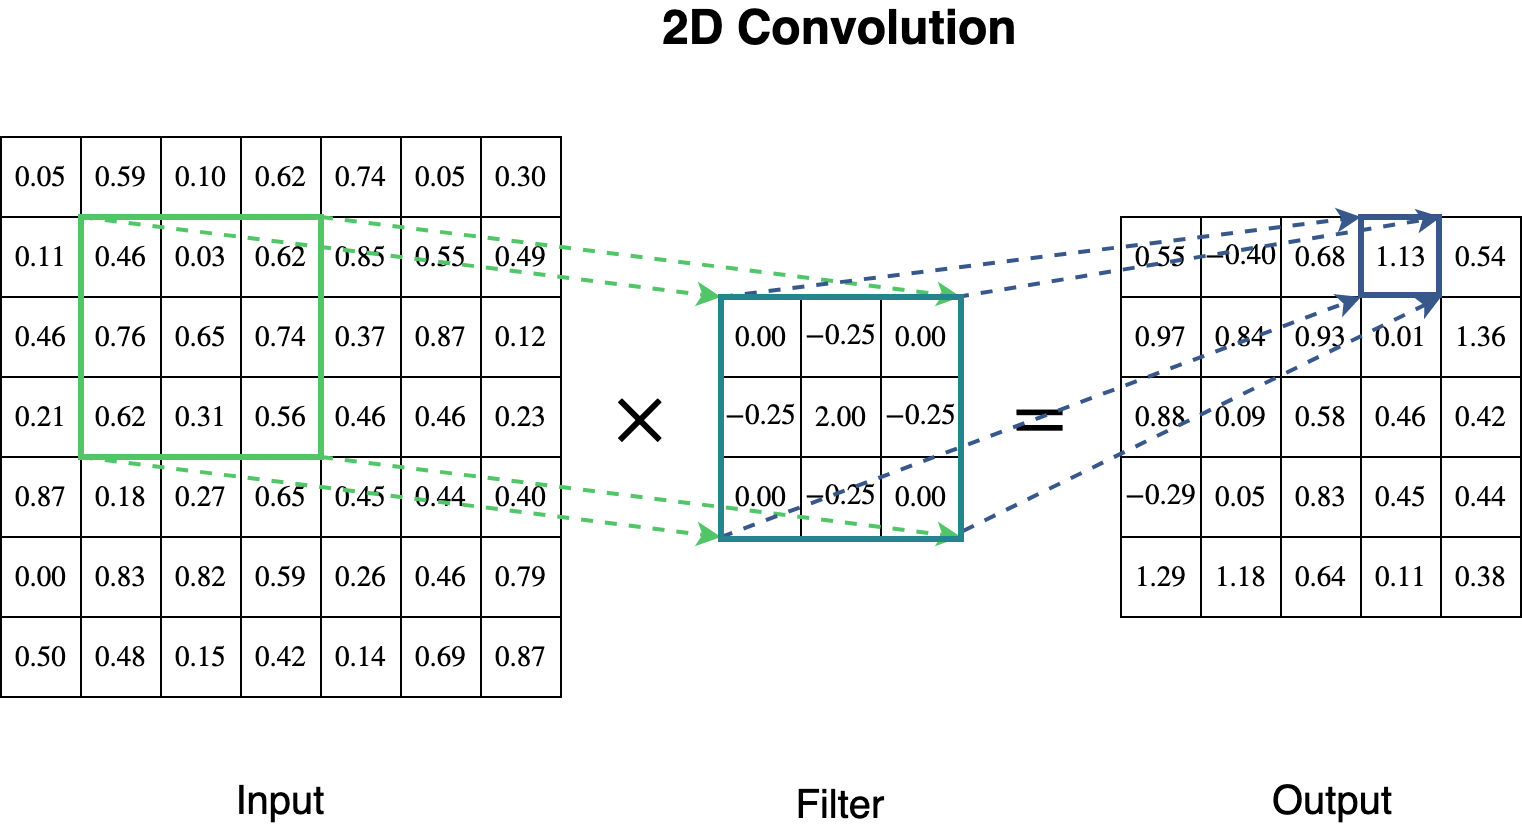
\includegraphics[width=1.0\textwidth]{img/convolution.png}
        	%\caption{}
        	\label{fig:convolution}
        \end{figure}
    \end{frame}
    
    \begin{frame}{Methods and Models | LSTM}
        \begin{figure}[hbt]
        	\center
        	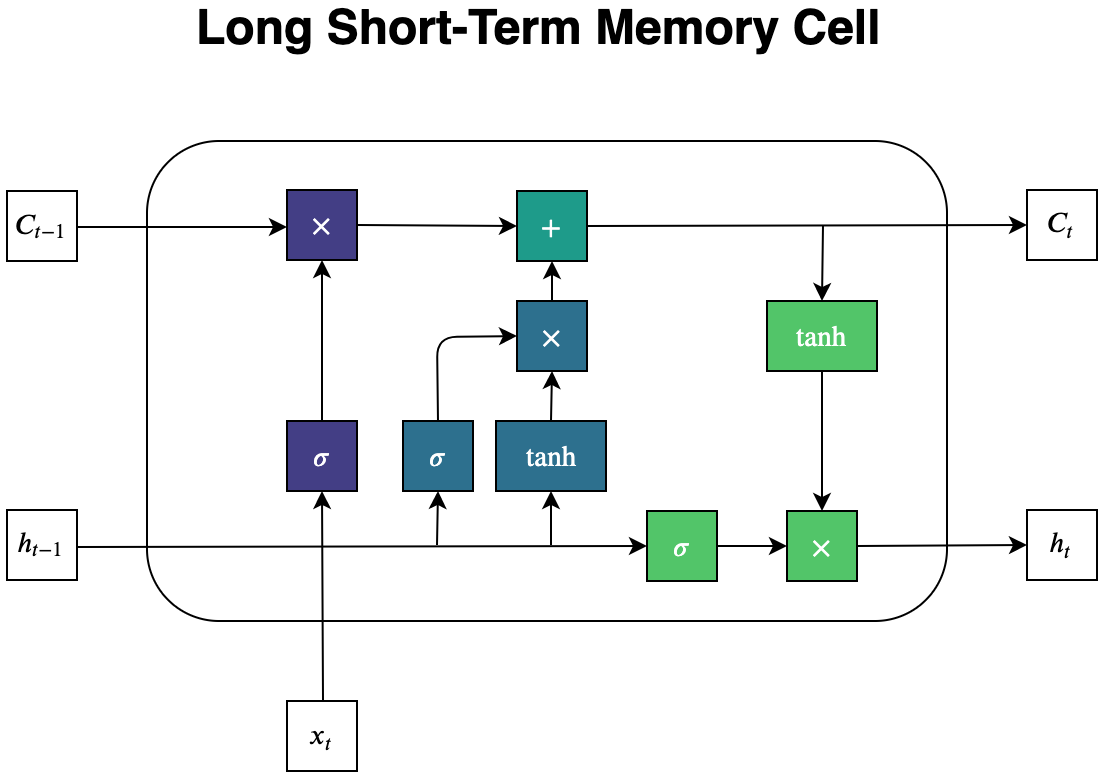
\includegraphics[width=1.0\textwidth]{img/LSTM-detailed.png}
        	%\caption{}
        	\label{fig:lstm_detailed}
        \end{figure}
    \end{frame}
    
    \begin{frame}{Methods and Models | DeepSleep}
        \begin{figure}[hbt]
        	\center
        	\includegraphics[width=0.5\textwidth]{img/deepsleep_part1.png}
        	%\caption{}
        	\label{fig:deepsleep}
        \end{figure}
    \end{frame}
    
        \begin{frame}{Methods and Models | DeepSleep}
        \begin{figure}[hbt]
        	\center
        	\includegraphics[width=0.7\textwidth]{img/deepsleep_part2.png}
        	%\caption{}
        	\label{fig:deepsleep}
        \end{figure}
    \end{frame}
    
    \section{Results}
    \begin{frame}{Results | Gdańsk}
        \begin{table}[h]
        \tiny
        \begin{tabular}{lrrrrr}
            \textbf{Gdańsk} & \textbf{Naive Bayes} & \textbf{Random Forest} & \textbf{SVM} & \textbf{XGBoost} & \textbf{DeepSleep} \\ \hline
            \multicolumn{6}{@{}l}{} \\
            \textbf{Regression / Complete} & \multicolumn{5}{@{}l}{}\\
            Training & & 57.64\% & 13.19\% & 32.64\% & 18.52\% \\ 
            Validation & & & & & 19.44\% \\
            Testing & & 27.03\% & \textbf{32.43\%} & 29.73\% & 24.32\% \\ \hline
            \multicolumn{6}{@{}l}{} \\
            \textbf{Regression / Constant} & \multicolumn{5}{@{}l}{}\\
            Training & & 71.35\% & 13.19\% & 24.35\% & 15.74\% \\
            Validation & & & & & 11.11\% \\
            Testing & & 25.84\% & \textbf{32.43\%} & 23.25\% & 29.73\% \\ \hline
            \multicolumn{6}{@{}l}{} \\
            \textbf{Classification / Complete} & \multicolumn{5}{@{}l}{}\\
            Training & 32.64\% & 100.00\% & 20.14\% & 100.00\% & 22.22\% \\
            Validation & & & & & 13.89\% \\
            Testing & 29.73\% & \textbf{32.43\%} & 10.81\% & 27.03\% & 10.81\% \\ \hline
            \multicolumn{6}{@{}l}{} \\
            \textbf{Classification / Constant} & \multicolumn{5}{@{}l}{}\\
            Training & 21.53\% & 100.00\% & 18.75\% & 99.31\% & 22.22\% \\
            Validation & & & & & 13.89\% \\
            Testing & 27.03\% & \textbf{32.43\%} & 5.41\% & 27.03\% & 10.81\% \\ \hline
        \end{tabular}
        %\caption{Results of the different classifiers on the data set providing by the University of Gdańsk.}
        \label{tab:results_gdansk}
        \end{table}
    \end{frame}
    
    \begin{frame}{Results | Physionet}
    \begin{table}[h]
    \tiny
    \begin{tabular}{lrrrrr}
        \textbf{Physionet} & \textbf{Naive Bayes} & \textbf{Random Forest} & \textbf{SVM} & \textbf{XGBoost} & \textbf{DeepSleep} \\ \hline
        \multicolumn{6}{@{}l}{} \\
        \textbf{Regression / Complete} & \multicolumn{5}{@{}l}{}\\
        Training & & 76.44\% & 40.20\% & 27.09\% & 25.36\% \\ 
        Validation & & & & & 29.87\% \\
        Testing & & 35.48\% & 29.68\% & \textbf{38.71\%} & 30.32\% \\ \hline
        \multicolumn{6}{@{}l}{} \\
        \textbf{Regression / Constant} & \multicolumn{5}{@{}l}{}\\
        Training & & 78.64\% & 11.74\% & 27.62\% & 39.79\% \\
        Validation & & & & & 42.20\% \\
        Testing & & 30.04\% & 29.03\% & 29.56\% & 32.90\% \\ \hline
        \multicolumn{6}{@{}l}{} \\
        \textbf{Classification / Complete} & \multicolumn{5}{@{}l}{}\\
        Training & 15.35\% & 99.78\% & 39.91\% & 99.78\% & 39.55\% \\
        Validation & & & & & 37.66\% \\
        Testing & 12.90\% & 29.03\% & 25.81\% & 27.10\% & \textbf{38.10\%} \\ \hline
        \multicolumn{6}{@{}l}{} \\
        \textbf{Classification / Constant} & \multicolumn{5}{@{}l}{}\\
        Training & 13.62\% & 99.78\% & 27.55\% & 51.22\% & 39.38\% \\
        Validation & & & & & 33.77\% \\
        Testing & 12.65\% & 33.68\% & 28.13\% & 33.94\% & \textbf{42.58\%} \\ \hline
    \end{tabular}
    %\caption{Results of the different classifiers on the data set provided by Physionet.}
    \label{tab:results_gdansk}
    %\end{adjustwidth}
    \end{table}
    \end{frame}
    
    \begin{frame}{Results | Physionet}
        \begin{figure}[hbt]
        	\center
        	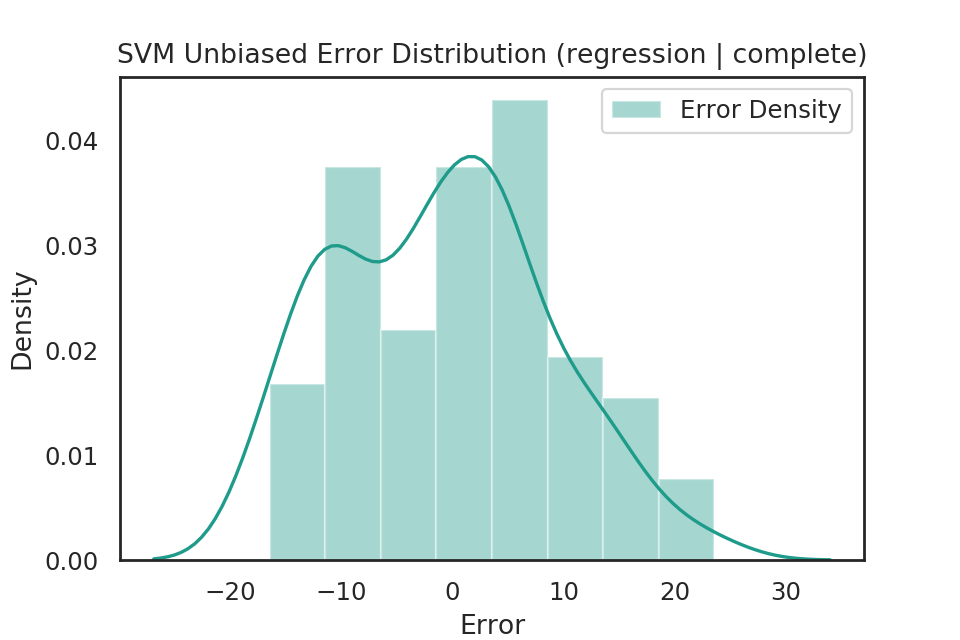
\includegraphics[width=1.0\textwidth]{img/physionet_svm_regression_complete_error_distribution_unbiased.png}
        	%\caption{}
        	\label{fig:example_error_distribution}
        \end{figure}
    \end{frame}
    
    \section{Data Simulation}
     \begin{frame}{Data Simulation | Gaussian Processes}
     
        A Gaussian Process is defined as
     
        \begin{equation}
            f(x) \sim \mathcal{GP}\big(m(x), k(\chi, \chi)\big)
        \end{equation}
        
        The whole statistical model is then defined as
        
        \begin{equation}
            y = \mathcal{N}\big(f(x), \sigma_{\text{noise}}\big)
        \end{equation}
    \end{frame}
    
    \begin{frame}{Data Simulation | Gaussian Processes}
    
    The joint of observations and points to predict is defined as
    
        \begin{equation}
            \begin{bmatrix}
            y \\
            f(x^\ast)
            \end{bmatrix}
            \sim
            \mathcal{N} \Bigg(m(x),
                \begin{bmatrix}
                k(\chi, \chi) + \sigma_{\text{noise}}^2I & k(\chi, \chi^\ast) \\
                k(\chi^\ast, \chi) & k(\chi^\ast, \chi^\ast)
                \end{bmatrix}
            \Bigg)
        \end{equation}
    \end{frame}
    
    \begin{frame}{Data Simulation | Gaussian Processes}
    
    Then we condition on the observations to obtain the predictive distribution
    
    \begin{equation}
        \label{eq:gp_fitted}
        \begin{split}
             f(x^\ast) | \chi^\ast, \chi, f(x) \sim \mathcal{N} \big(
            \bar{f_\ast}, \text{cov}(f_\ast)
            \big)
        \end{split}
        \end{equation}
        
        \begin{equation}
            \label{eq:gp_fitted_mean}
            \bar{f_\ast} = k(\chi^\ast, \chi) \big(k(\chi, \chi) + \sigma_{\text{noise}}^2I\big)^{-1}y
        \end{equation}
        
        \begin{equation}
            \label{eq:gp_fitted_covariance}
            \text{cov}(f_\ast) = k(\chi^\ast, \chi^\ast) - k(\chi^\ast, \chi) \big( k(\chi, \chi) + \sigma_{\text{noise}}^2I \big)^{-1} k(\chi, \chi^\ast)
        \end{equation}
    \end{frame}
    
    \begin{frame}{Data Simulation | GP | Point Estimates}
    
    Optimise the log likelihood proportion, with respect to each parameter in $\theta$
    
    \begin{equation}
        \mathcal{L}(y | X, \theta) \propto - \frac{1}{2}y^T \big(K_\theta + \sigma_{\text{noise}}^2I\big)^{-1}y - \frac{1}{2} \log{|K_\theta + \sigma_{\text{noise}}^2I|}
    \end{equation}
    \end{frame}
    
    \begin{frame}{Data Simulation | GP | Point Estimates}
    \begin{figure}[hbt]
        	\center
        	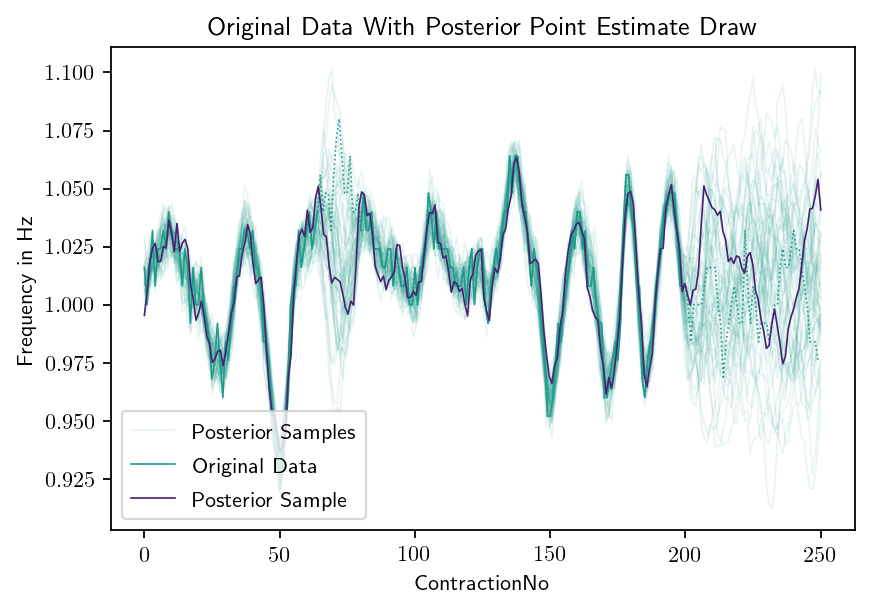
\includegraphics[width=1.0\textwidth]{img/gp_data_example_posterior_gradient_descent.png}
        	%\caption{}
        	\label{fig:posterior_point_estimaes}
        \end{figure}
    \end{frame}
    
    \begin{frame}{Data Simulation | GP | Posterior Predictive Distribution}
    
        The posterior predictive distribution is given as
    
        \begin{equation}
            p(\Tilde{y}|y) = \int_\theta p(\Tilde{y}|\theta, y) p(\theta|y)d\theta
        \end{equation}
    
        Update parameters for each slice, as
        
        \begin{equation}
            p(\theta|\chi_a,\chi_b) \propto p(\chi_b|\theta)p(\theta|\chi_a)
        \end{equation}
    \end{frame}
    
    \begin{frame}{Data Simulation | GP | Posterior Predictive Distribution}
        \begin{figure}[hbt]
        	\center
        	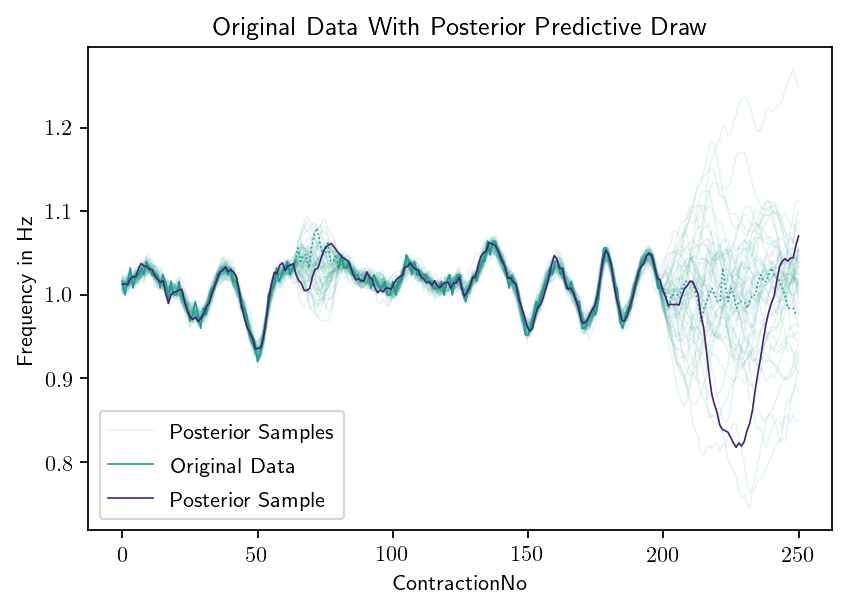
\includegraphics[width=1.0\textwidth]{img/gp_data_example_posterior_predictive.png}
        	%\caption{}
        	\label{fig:posterior_predictive_kernel}
        \end{figure}
    \end{frame}

     \begin{frame}{Data Simulation | GP | Posterior Predictive Distribution}
        \begin{figure}[hbt]
        	\center
        	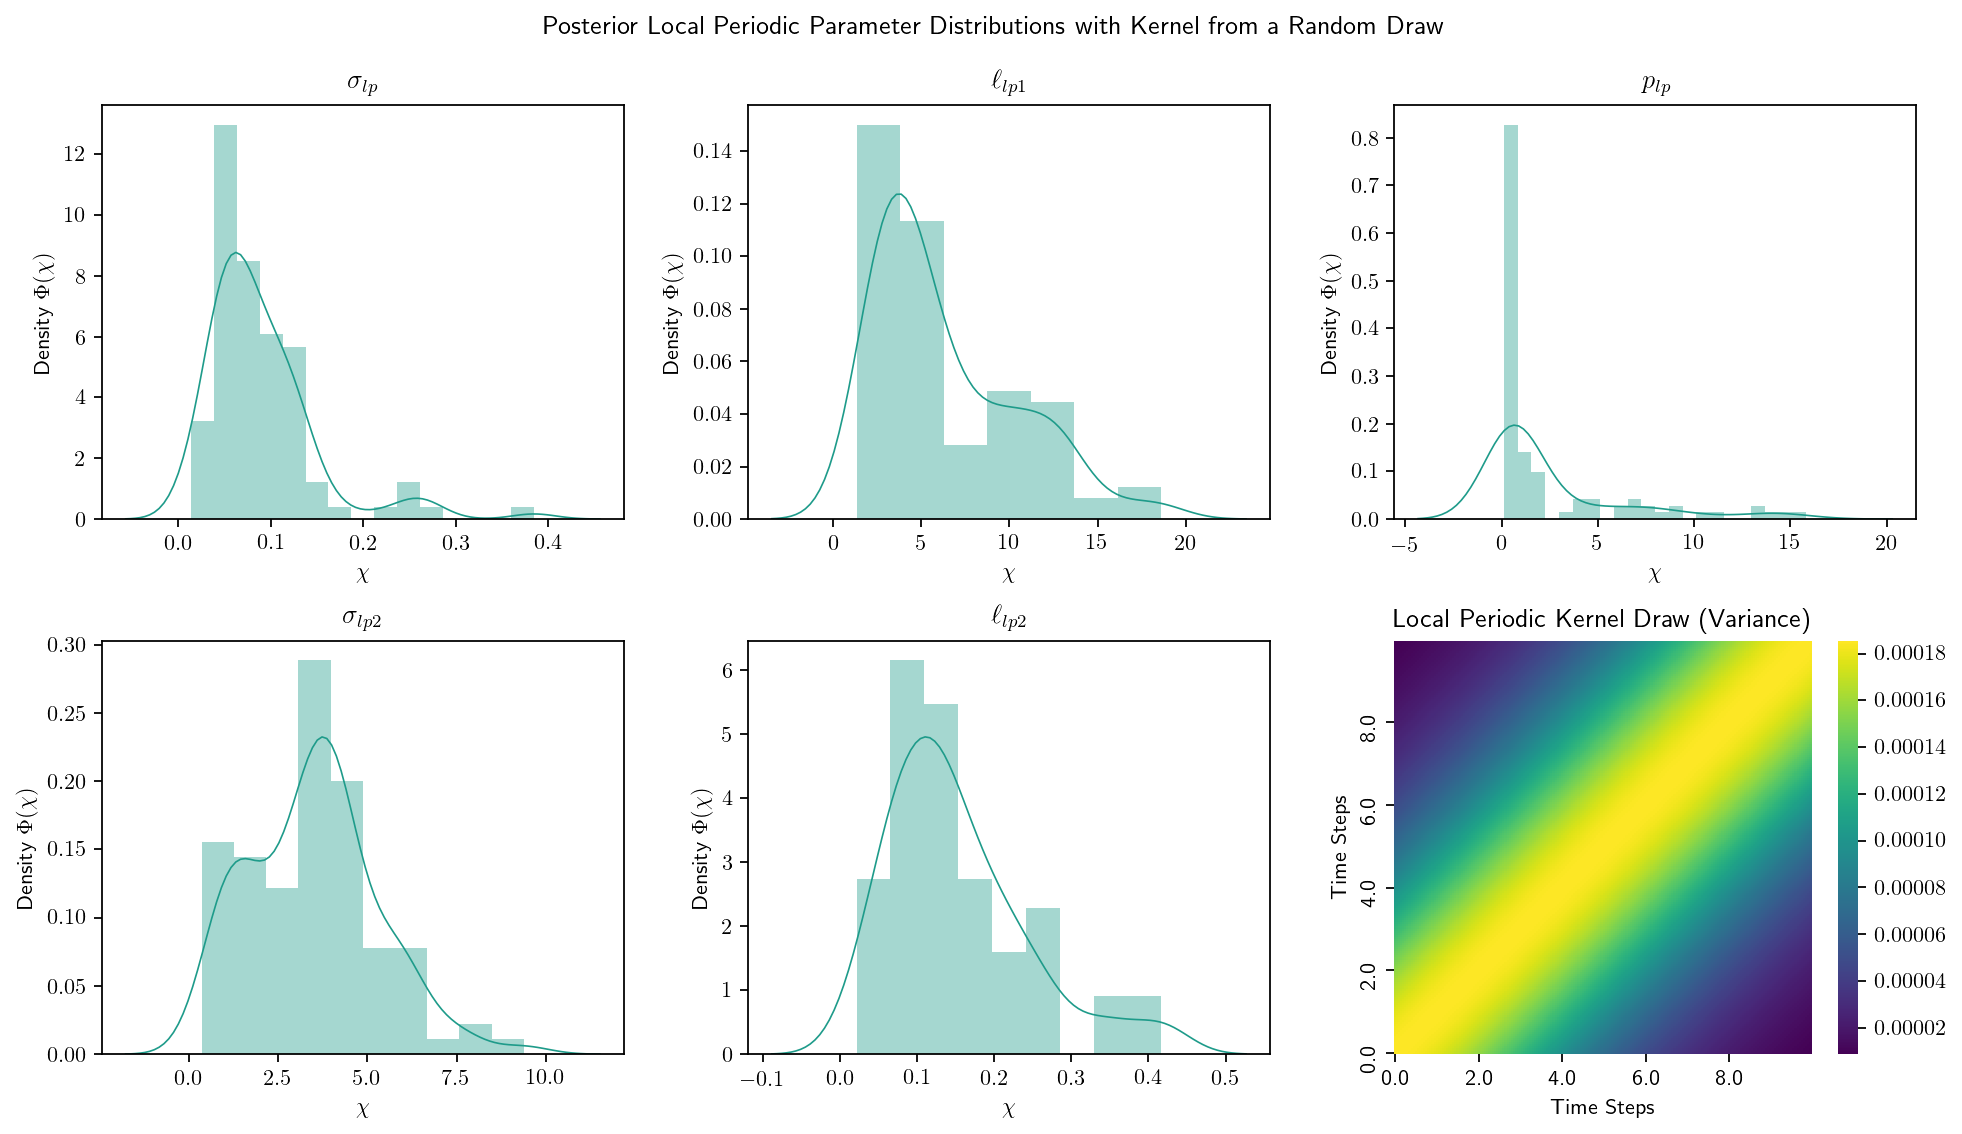
\includegraphics[width=1.0\textwidth]{img/gp_kernel_posterior_local_periodic_zoomed.png}
        	%\caption{}
        	\label{fig:posterior_predictive_kernel}
        \end{figure}
    \end{frame}
    
    \section{Status and Outlook}
    \begin{frame}{Status and Outlook}
        \begin{itemize}
            \item Bayesian simulation is currently running
            \item For comparison: point estimates
            \begin{itemize}
                \item Numerical solution already implemented, but takes a lot of time
                \item Maybe solving analytically
            \end{itemize}
            \item Evaluate models on simulated data
            \item Analyse results
        \end{itemize}
    \end{frame}
    
    \appendix
    
    \begin{frame}[standout]{}
        \center Appendix
    \end{frame}
    
    \begin{frame}[allowframebreaks]{References}
    
      \bibliography{literature.bib}
      \bibliographystyle{apalike}
    
    \end{frame}
    
\end{document}